% !TeX spellcheck = en_US
\section{Introduction}\label{sec:Intro}

For the first time in decades, numerous countries world-wide, including the United States, are facing high inflation rates. This is important because households generally perceive high inflation as one of the most important (economic) policy issues \citep{Shiller.1997, Stantcheva.2024}. While some inflation might be desirable, rates way above the two percent target impose substantial costs on society \citep{Romer.2012}. Consequently, its origin and the underlying mechanisms have been and continue to be subject of ongoing debate. \cite{Blanchard.2023} attribute the increase in inflation to a combination of supply constraints and robust aggregate demand. \cite{Reis.2022} highlights an ``overly long period of expansionary policy'', and central banks tolerating higher inflation rates. \cite{Weber.2023} discuss the role of market power to hike prices, which indicates ``sellers' inflation''. On a theoretical level, \cite{Werning.2023} provide a decomposition of inflation and argue that the general cause of inflation is conflict or disagreement. Expectations are of great importance in their conceptualization, as they shape the aspirations of workers and firms.

%\begin{figure}[H]
%	\centering
%	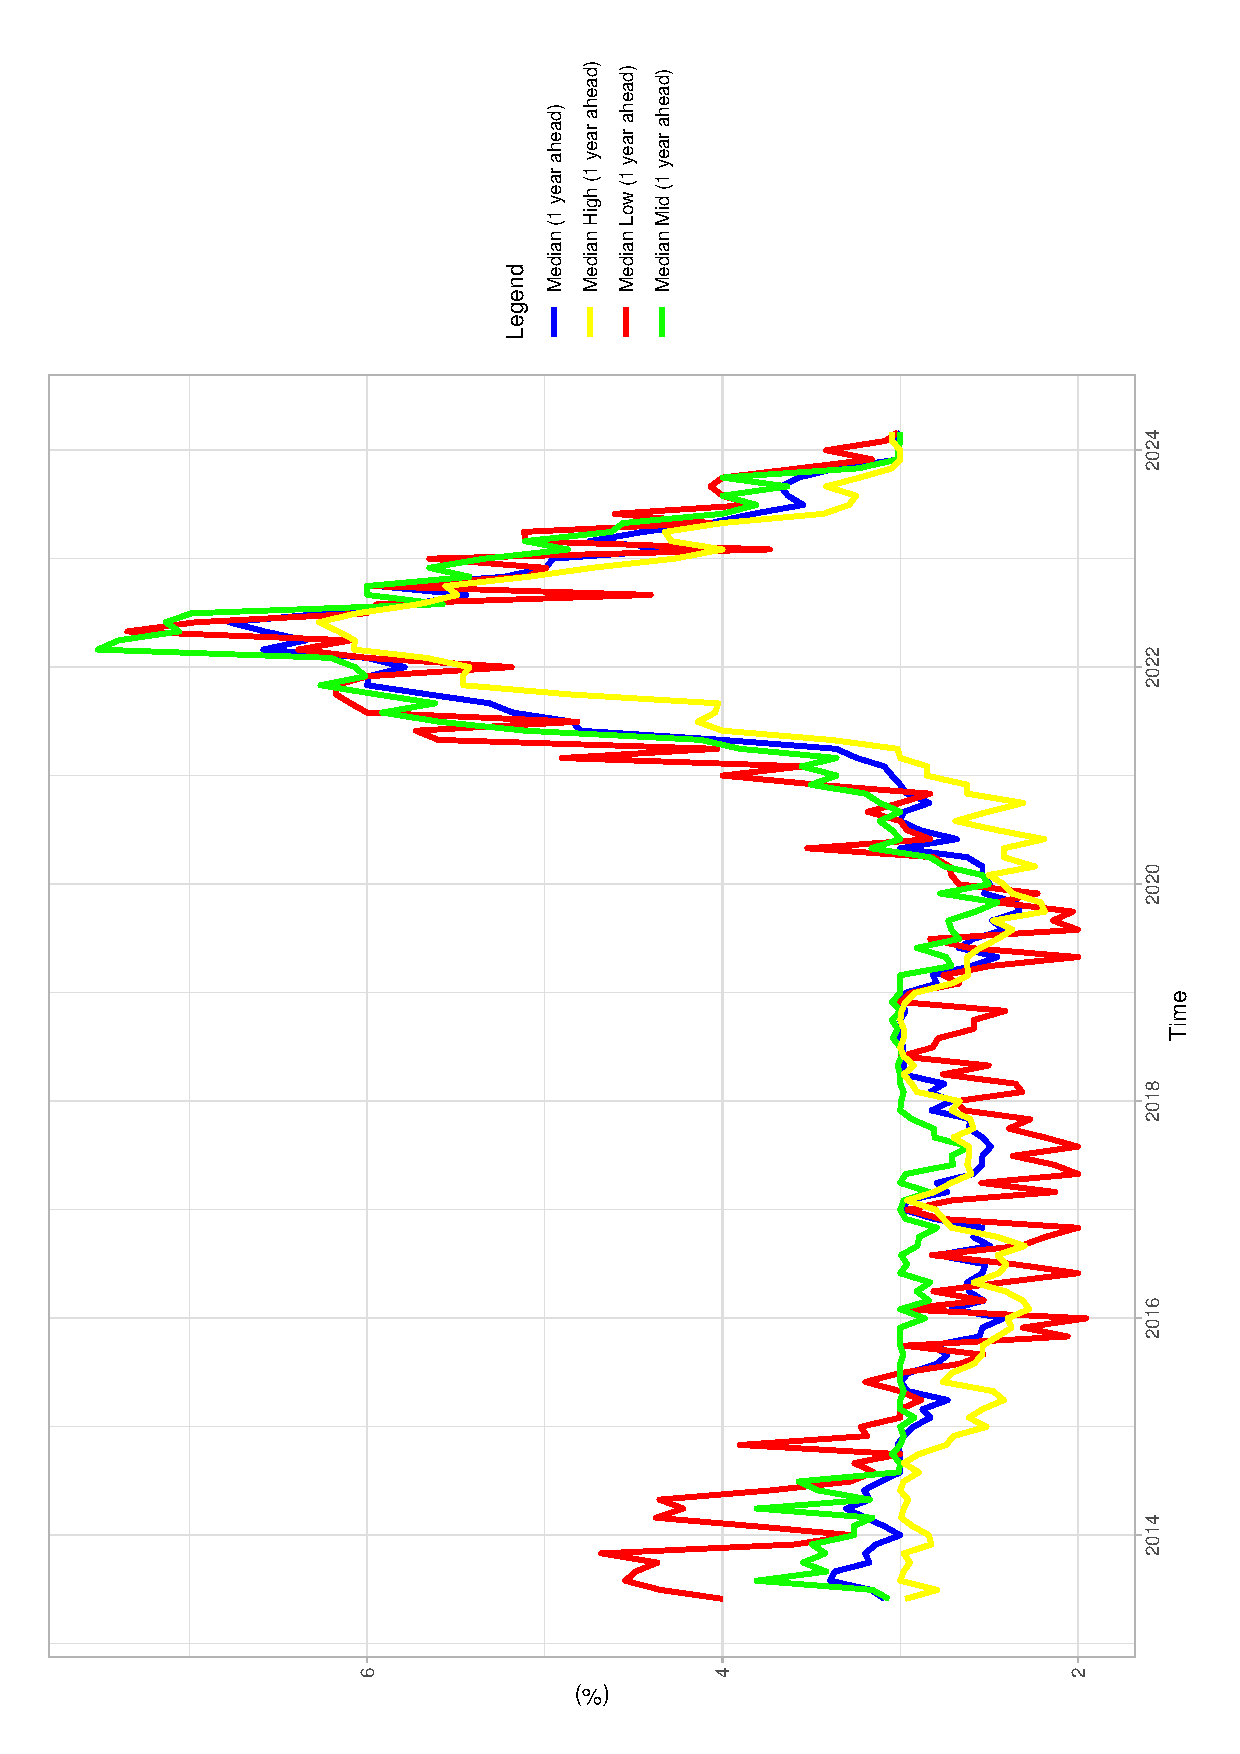
\includegraphics[width=0.95\linewidth]{figures/infl_expect.png}
%	\caption{Median inflation expectations of US households}
%	\label{fig:inflexpect}
%	\floatfoot{Note: Median survey-based inflation expectations of US households one and three years ahead. Source: New York Fed Survey, see \cite{Armantier.etal.2017} for details.} 
%\end{figure}

In standard New Keynesian models, this idea of forward-looking agents is essential, as \cite{Werning.2022} demonstrates. In these models, expectations are seen as a driver of inflation dynamics. Influential on forward-guidance was the work by \cite{Krugman.1998}, who proposed that during a liquidity trap, central banks should be able to stimulate the economy by raising inflation expectations through credibility. This is why central banks closely monitor the expectations of households, firms, and experts— or, as Jerome Powell, the current Chair of the Federal Reserve, puts it: ``Our monetary policy framework emphasizes the importance of well-anchored inflation expectations, both to foster price stability and to enhance our ability to promote our broad-based and inclusive maximum employment objective.'' \citep{Powell.2021}. 

A long tradition of empirical economic research addresses the question of whether and to what extent the expectations of households influence economic decisions. Two moments are subjects of interest: the consumption-saving nexus in the Euler-Equation and inflation uncertainty as a precautionary saving motive \citep{DAcunto.2023}. Regarding the former, work by \cite{Juster.1972} suggested already in the 1970s that inflation expectations influence expenditure spent on durable goods, while the findings fo \cite{Burch.1975} indicate a strong relationship between inflation expectations and the national saving rate. More recent research by \cite{Bachmann.2015} is also in line with both moments. The authors do report a significant negative relationship between expectations and savings, but only for a subset of households, whose expectations are within one percentage point of the actual realized inflation. By linking survey data on inflation expectations of households to administrative data, \cite{Vellekoop.2019} report a negative relationship between inflation expectations and net worth. With a pseudo-panel study, the results of \cite{Duca.2021} are in line with the Euler equation for all participants, however, smaller effect sizes for more inaccurate expectations. Further supporting evidence comes from \cite{Draeger.2021}, who report positive correlation between current spending and inflation expectations for a German sample. Their results further indicate the importance of attention to monetary news as an amplifier of this channel. However, regarding the actual spending, the findings by \cite{Burke.2023} suggest that the expectation effect applies only to spending on durable goods. 

While the introduction of rational expectations by \cite{Muth.1961}, \cite{Lucas.1972}, \cite{Lucas.1979} led to a revolution in economic modeling, the last two decades have been marked by strong criticism of the ``full information rational expectations'' (FIRE) model \citep{Coibion.Gorodnichenko.2012}. Alternative approaches to the formation of expectations include ``sticky information'' \citep{Mankiw.2002,Carroll.2003,Carroll.2005, doepke.etal.2008a, doepke.etal.2008b}, ``rational inattention'' \citep{Woodford.2001, Sims.2003}, ``learning'' \citep{Evans.Honkapohja.2001} and ``bounded rationality'' \citep{Gabaix.2014, Fuster.2010, Evans.Honkapohja.2001}. Regarding the heterogeneity of expectations, \cite{Weber.etal.2022} identify four different channels that affect subjective inflation expectations: 
\begin{enumerate}
	\item Exposure to heterogeneous price signals \citep{Acunto.2021},
	\item different media information sets \citep{Carroll.2003,Carroll.2005, doepke.etal.2008a,Bachmann.2021,DAcunto.2022a,Draeger2016},
	\item cognitive ability, education, and the usage of heuristics \citep{DAcunto.2019a, DAcunto.2022b, Gennaioli.2010}, and
	\item heterogeneous incentives to obtain information \citep{Cavallo.2017}.
\end{enumerate}

This observed heterogeneity and subjectivity of inflation expectations is largely undisputed nowadays, however, there is still no consensus in economics as to what determines these expectations. To some extent, ``narrative economics'' \citep{Shiller.2017,Shiller.2019} has created a link to modern social science and psychological analysis of expectations and uncertainty \citep{Beckert.2016, Bronk.2018, Tuckett.2017}. The theoretical argument is based on findings from literary studies, sociology, anthropology, and psychology that highlight the importance of narratives for human beings and human decision-making \citep{Shiller.2017}. It states that narratives about the economy pervade and guide decisions in uncertain moments. Therefore, they incorporate ``[...] causal, temporal, analogical, and valence information about agents and events, which serve to explain data, imagine and evaluate possible futures, and motivate and support action over time'' \citep{Johnson.2023}. This highlights the importance of expectations, i.e. narratives for imagining and evaluating the future \citep{Johnson.2023, Bronk.2018}.

In microeconomic models \citep{Eliaz.2020, Eliaz.2022}, the narrative approach has been implemented, establishing a connection with the statistical and epistemological literature on causality \citep{Pearl.2009}. \cite{Eliaz.2020} refer to political debates and suggest that actors are encouraged to strategically adopt political stances aligned with narratives, which both perceive to have more positive and promising outcomes. From a macroeconomic perspective, \cite{Shiller.2017,Shiller.2019} emphasizes the  role of ``going viral'' for narratives by focusing on the spread and dynamic of economic narratives. Following \cite{Shiller.2019}, this aspect is crucial because narratives are closely linked to ``animal spirits'' \citep[17]{Shiller.2009}. Thus, viral narratives may lead to fundamental shifts and turning points, being active drivers of the economy and of activity in the economy \citep{reccius.2024}. Research should therefore focus on the spread and dynamics of economic narratives.

%Since the work of \cite{Shiller.2017,Shiller.2019} the strand of ``narrative economics'' has gained momentum. Nevertheless, research about narratives in context of inflation and inflation expectations remains scare. 

In a recent paper, \cite{Andre.2023} take the existing strand of research on expectations and link it to the strand of ``narrative economics'': Based on a working definition of economic narratives as ``causal accounts of past economic events'' \citep[5]{Andre.2023}, the authors focus on measuring backward-looking narratives through open-ended questions. In order to classify narratives, the authors use the concept of ``directed acyclic graphs'' (DAG) \citep{Pearl.2009}. Their findings suggest that narratives among households substantially differ from those of experts. This is partly explained by different political attitudes and news consumption. Moreover, they provide experimental evidence that expectations respond to narrative priming and that mass media is an important source of narratives.

The relevance of the media as an intermediary of narratives \citep{Ellen.2022} is considered by some empirical research. \cite{Larsen.2021} analyze news coming from the Dow Jones Newswire by means of a Latent Dirichlet Allocation (LDA) model \citep{blei.2003}.  Their results suggest that media news reports are a good predictor of inflation expectations. \cite{Mueller.2022} use an augmented version of the static LDA, which allows for a dynamic analysis of news about inflation in German newspapers, yet without considering them as determinants of expectations. Related work comes from \cite{Hong.2022}, who combines LDA modeling with forecasting techniques. \cite{Macaulay.2022} measure narratives by means of LDA on social media and investigate their effects on consumer sentiments with a high-frequency event study. All these papers have one aspect in common: They rely on (dynamic) exploratory LDA topic models to measure narratives in the media, which limits their methodological approach to a broad definition of narratives. Therefore, the previous approaches were unable to identify concrete predefined concepts of narratives \citep{reccius.2024}. 

Building upon the existing research, this paper addresses the following research objectives:

\begin{enumerate}
	\item Provide a methodological approach that goes beyond existing research to identify narratives in large text corpora and enables researchers to measure their prevalence according to predefined concepts.
	\item Focus on the predominant inflation narratives in media reports during the recent inflationary period. 
	\item  Investigate if inflation narratives are potential causal determinants of expectations.  
	\item Finally, this paper examines whether certain narratives have a stronger impact on certain socio-economic groups (e.g. by income, education, age, numeracy) than other narratives. 
\end{enumerate}

In order to do that, the paper utilizes the existing methodological approach to measure narratives a step further and proposes a combination of results coming from the survey study by \cite{Andre.2023} and a ``keyword-assisted topic model'' (\textsf{keyATM}) in a variant called ``dynamic \textsf{keyATM}'', proposed by \cite{Eshima.2023}. This allows us to provide prior information about the narratives into the Bayesian estimation. This novel method overcomes the common problem of measuring specific concepts while using explorative topic models, e.g. LDA by \cite{blei.2003}; it enables the researcher to specify a number of keywords to label topics prior to fitting the model on the data. For our purpose, we construct thirteen keyword-specified topics, that incorporate demand and supply narratives, as well as miscellaneous narratives, e.g., pandemic or war narrative, based on the findings by \cite{Andre.2023}. We refine our measurements by applying a Latent Semantic Scaling (\textsf{LSS}) technique \citep{Watanabe.2021} to identify the direction of the narratives' argument and to construct corresponding indices. To investigate their predictive power over macroeconomic variables, we conduct multivariate Granger causality tests. Further, we study the diffusion of each narrative by applying ``local projections'' techniques \citep{Jorda.2005}.

Our empirical findings suggest that during the current inflationary period, narratives about monetary policy, demand shifts, supply chain issues, energy prices, labor shortages, corporate profits, and the pandemic as causes of rising inflation were highly significant. Moreover, stories about the war in Ukraine showed a sudden and strong increase, which, however, did not persist. As our time series analysis indicates, many of these narratives contain predictive power for short- and medium-term household inflation expectations. Our analysis highlights the importance of narratives surrounding government spending, supply chains, labor shortages, war, and corporate profits in shaping household inflation expectations. Supplementary, by analyzing the impulse responses of a shock in the narratives, we provide evidence that narrative diffusion elevates households' inflation expectations, 1-year-ahead expectations in particular. When comparing shocks across narratives, we notice more anchored expectations with respect to a shock in the supply chain, demand shift, and profits narratives. Along the various socioeconomic determinants, such as income, education, age, etc., we find clear differences in the way narratives affect inflation expectations. For example, our analysis indicates that the energy and profits narratives are the main driver of medium-term expectations for households with lower annual incomes, while we find more Granger causalities for middle- and high-income households, including several demand narratives. This suggests a strong group-specific susceptibility to narratives and underlines the need for interdisciplinary (social science) analyses when it comes to explaining heterogeneous inflation expectations \citep{Beckert.2016}. Finally, our results emphasize the spread and change of narratives over a short period of time and highlight economic narratives as a determinant of expectation building.\\

The paper is structured as follows: Firstly, Section \ref{sec:MethodsData} briefly describes the datasets and some of the preceding pre-processing steps. Further, we provide a short overview of the narratives identified by \cite{Andre.2023} with corresponding pre-selected keywords, and further describe the applied empirical methods, namely \textsf{keyATM}, \textsf{LSS}, Granger causality tests, and local projections. Subsequently, section \ref{sec:Analysis} offers a first outline of the dynamic \textsf{keyATM} results. Secondly, we report results from the \textsf{LSS} and provide constructed indices of narratives. Lastly, we present estimation results from the Granger causality tests and local projections. Further background information, the Online Appendix and the replication code will be made available via a repository at \url{https://github.com/ValweM/InflationNarratives} \footnote{All calculations in the paper were performed using R software \citep{R.2022} version 4.4.1. The software is licensed under GPL-2/GPL-3. Furthermore Python version 3.12.2 \citep{python.2009} was used for several NLP pre-processing tasks (e.g lemmatization).}
